\documentclass[9pt]{beamer}

\usetheme[progressbar=frametitle,block=fill,background=light]{metropolis}
\usefonttheme{serif}

\usepackage{appendixnumberbeamer}

\usepackage{booktabs}
\usepackage[scale=2]{ccicons}


\usepackage{pgfplots}
\usepgfplotslibrary{dateplot}
\usepackage{pgfplotsthemetol}
\usepackage{amsmath,amssymb,amsthm,amsfonts,amstext}
\usepackage{bbm}
\usepackage{array}

\usepackage{xspace}

\usepackage{import}
\import{}{Packages/custom_macros.tex}

\newcommand{\themename}{\textbf{\textsc{metropolis}}\xspace}
\renewcommand{\emph}{\alert}

\title{Group theory, Topology and Spin-$1/2$ Particles}
\subtitle{From Dirac's belt to fermions}
% \date{\today}
\date{}
\author{Louan Mol}
\institute{Unversité Libre de Bruxelles\\[2cm]{\small Brussels Summer School of Mathematics 2022}}
% \titlegraphic{\hfill\includegraphics[height=1.5cm]{logo.pdf}}

\begin{document}

\maketitle

\nocite{*}

\begin{frame}{Table of contents}
    \setbeamertemplate{section in toc}[sections numbered]
    \tableofcontents%[hideallsubsections]
\end{frame}

\section{Dirac's belt trick and rotations}

\begin{frame}{Dirac's belt trick}
    
    You need:
    \begin{itemize}
      \item a belt (not necessarily Dirac's)
      \item a heavy book
    \end{itemize}
    Rules:
    \begin{enumerate}
      \item you can only move the end of the belt
      \item you cannot twist or rotate it
    \end{enumerate}
    \textbf{Goal:} untwist a $2\pi$-twist.\\[0.5cm]
      $\Rightarrow$ it tuns out to be \emph{impossible} ! One turn negates the twist: $2\pi\to-2\pi$. \\[0.5cm]

      Therefore, possible for a $4\pi$ twist ...\\ \hspace{7cm} Why is that ?

\end{frame}

\begin{frame}{Space of rotations: $\SO(3)$ as a group}
      
      Rotations in $3$-dimensional space: matrices that acts on $\R^3$ s.t. 
      \begin{enumerate}
        \item preserve the \emph{scalar product}: $O^TO=\mathbbm{1}$ ($\Leftrightarrow$ $O$ is orthogonal)
        \item preserve the \emph{orientation}: $\det O=1$
      \end{enumerate}

      \begin{block}{Special othogonal group}
        $\SO(3)$ is the set of $3\times 3$ real matrices such that $O^TO=\mathbbm{1}$ and $\det O=1$.
      \end{block}
      Three ``fundamental'' rotations:
      \begin{equation*}
        {\tiny
        x:
        \begin{bmatrix}
          1 & 0 & 0 \\
          0 & \cos\theta & -\sin\theta \\
          0 & \sin\theta & \cos\theta
        \end{bmatrix}\qquad
        y:
        \begin{bmatrix}
          \cos\theta & 0 & -\sin\theta \\
          0 & 1 & 0 \\
          \sin\theta & 0 & \cos\theta
        \end{bmatrix}\qquad
        z:
        \begin{bmatrix}
          \cos\theta & -\sin\theta & 0 \\
          \sin\theta & \cos\theta & 0 \\
          0 & 0 & 1
        \end{bmatrix}}
      \end{equation*}

      $\Rightarrow$ It forms a \emph{group}.
    
\end{frame}

\begin{frame}{Space of rotations: $\SO(3)$ as a topological space}
    Fundamental data that describes a rotation:
    \begin{itemize}
      \item an \emph{axis} of rotation, i.e. a  unit vector $\overrightarrow{n}$ \hspace{1.07cm}\textcolor{blue}{$\to$ 2 parameters}
      \item an \emph{angle} of rotation $\theta\in[-\pi,\pi]$ (with $-\pi\sim\pi$) \textcolor{blue}{$\to$ 1 parameter}
    \end{itemize}
    The space of rotations can then alternately be defined as a \textbf{$\boldsymbol{3}$-sphere of radius $\boldsymbol{\pi}$ and its antipodal points identified}:
    

    \begin{columns}[T,onlytextwidth]
      \column{0.5\textwidth}
          \vspace{0.5cm}
          \begin{equation*}
            \boxed{\SO(3)\cong B^3(\pi)/\sim}
          \end{equation*}
          and for each point:
          \begin{align*}
              \text{direction} &\leftrightarrow \text{axis}\\
              \text{norm} &\leftrightarrow \text{angle}
          \end{align*}
          $\Rightarrow$ It forms a \emph{topological space}.
  
      \column{0.5\textwidth}
  
          \begin{figure}
              \centering
              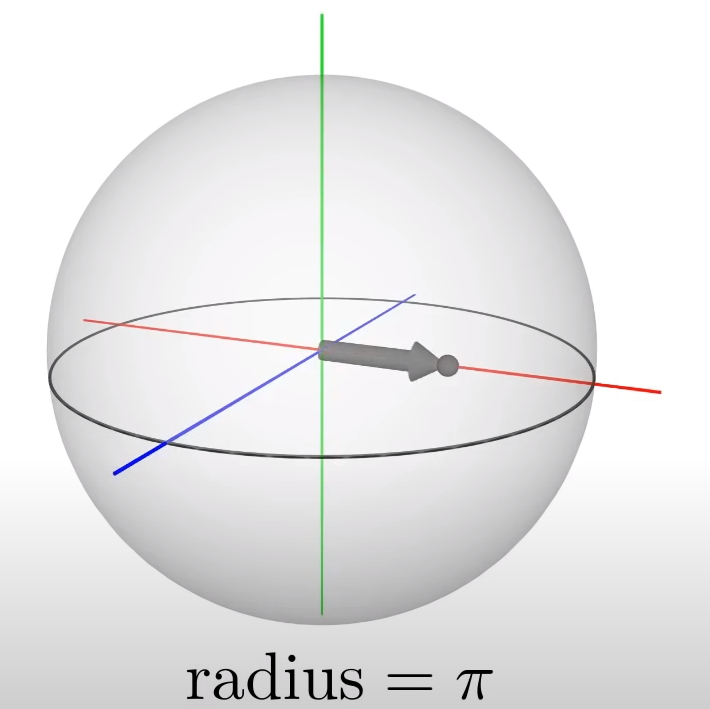
\includegraphics[scale=0.16]{Pictures/SO3sphere.png}
          \end{figure}
  
    \end{columns}

    (group $+$ topological space $=$ Lie group)
    
\end{frame}

\begin{frame}{Back to the belt}

    Mathematical description of the belt ?\\[0.3cm]
    \quad $\triangleright$ a belt is a strip, which is just a \emph{path} $+$ an \emph{orientation}.\\[0.2cm]
    \quad $\triangleright$ given axis on the middle line along the belt, each set of axis \\ \hspace{0.5cm} is related by a rotation \\[0.2cm]
    \quad $\triangleright$ a belt configuration is equivalent to a continuous set of axis and \\ \hspace{0.5cm} therefore to a continuous set of translations, i.e. a \emph{path in $\SO(3)$}
    \begin{figure}
        \centering
        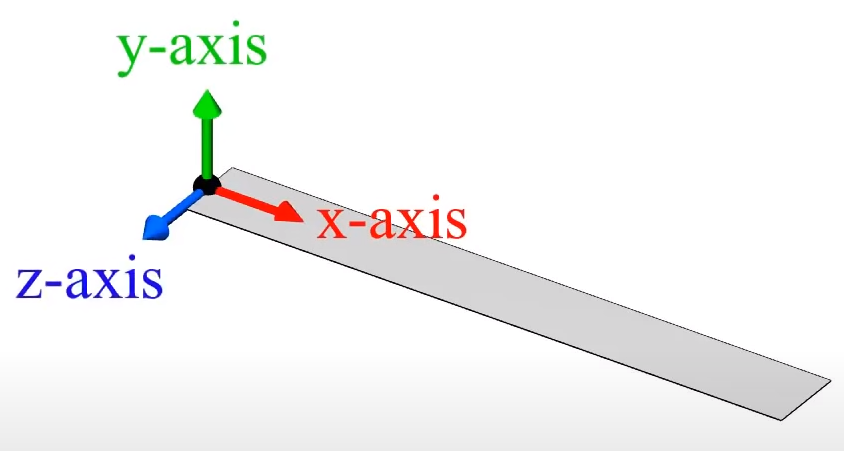
\includegraphics[scale=0.12]{Pictures/beltaxis.png}
    \end{figure}
    There is a bijection:
    \begin{equation*}
        \boxed{\text{belt configuration} \Leftrightarrow \text{path in $\SO(3)$}}
    \end{equation*}
    This gives us a new language to analyze the problem !

\end{frame}

\begin{frame}{Dictionary}
      \makebox[315pt][r]{
        \begin{tabular}{cccc}
            \textbf{\underline{trivial rotation}} & \textbf{\underline{$2\pi$ \textcolor{red}{$x$}-rotation}} & \textbf{\underline{$2\pi$ \textcolor{green}{$y$}-rotation}} & \textbf{\underline{$2\pi$ \textcolor{blue}{$z$}-rotation}}\\
            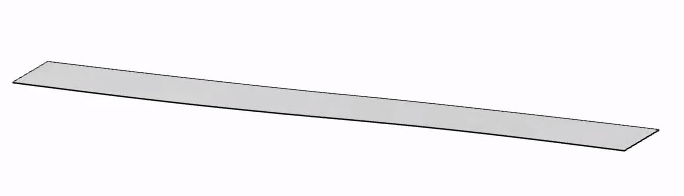
\includegraphics[scale=0.12]{Pictures/flatbelt.png} & 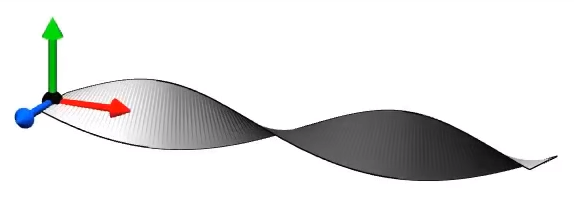
\includegraphics[scale=0.12]{Pictures/xaxisbelt.png} & 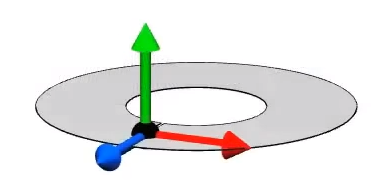
\includegraphics[scale=0.15]{Pictures/yaxisbelt.png} & 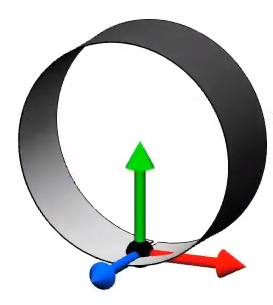
\includegraphics[scale=0.15]{Pictures/zaxisbelt.png} \\
            $\updownarrow$ & $\updownarrow$ & $\updownarrow$ & $\updownarrow$ \\
            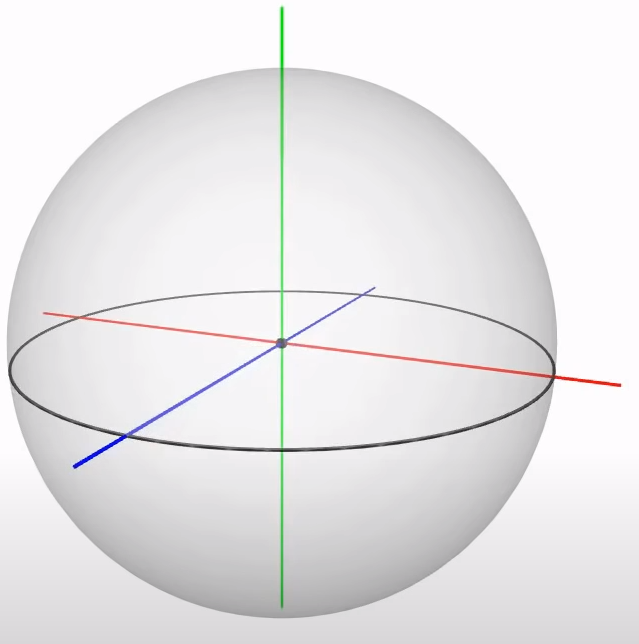
\includegraphics[scale=0.1]{Pictures/4pisphere4.png} & 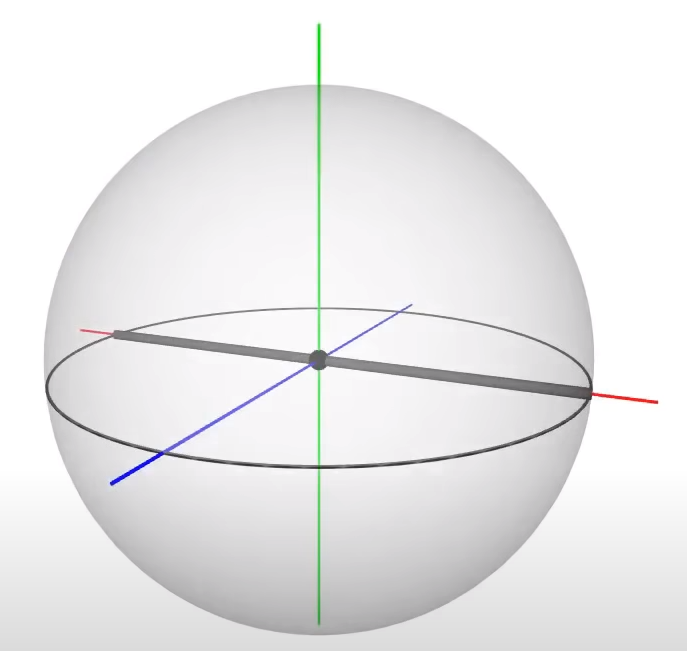
\includegraphics[scale=0.1]{Pictures/xaxissphere.png} & 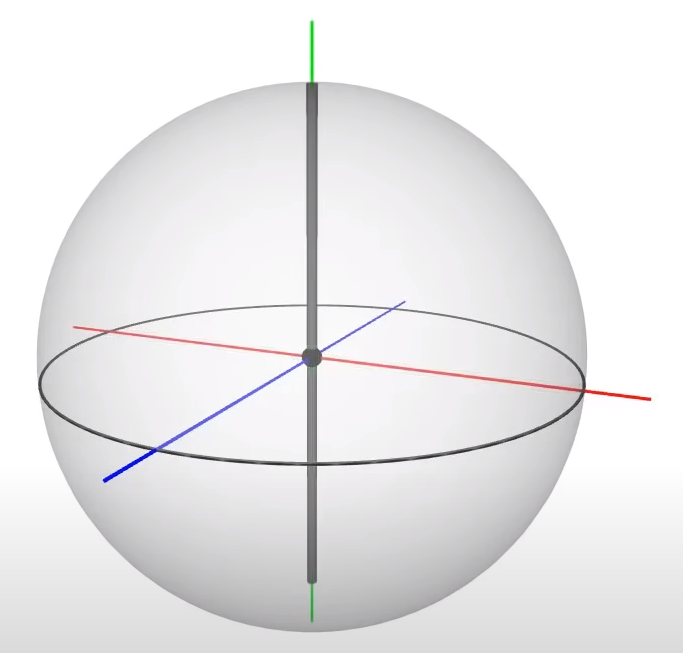
\includegraphics[scale=0.1]{Pictures/yaxissphere.png} & 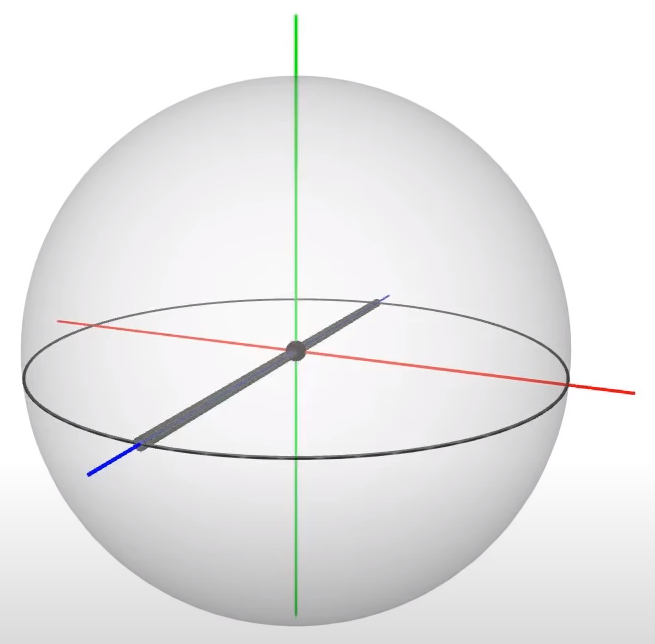
\includegraphics[scale=0.1]{Pictures/zaxissphere.png}
        \end{tabular}}
\end{frame}

\begin{frame}{Dictionary}
    \begin{center}
    \begin{tabular}{ccc}
        \textbf{\underline{random rotation}} & \textbf{\underline{closed}} & \textbf{\underline{open path}}\\
        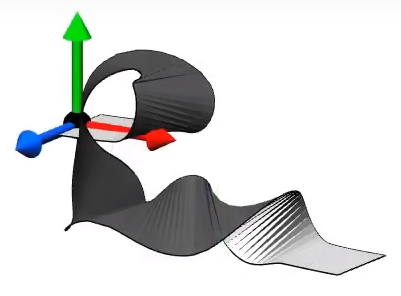
\includegraphics[scale=0.15]{Pictures/randomrotbelt.png} & 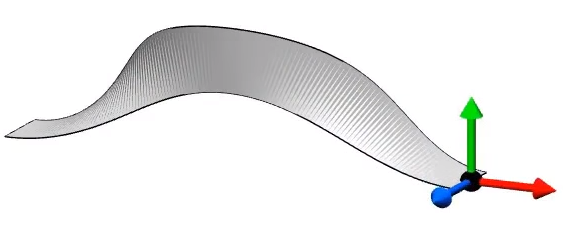
\includegraphics[scale=0.1]{Pictures/contractiblepathbelt.png} & 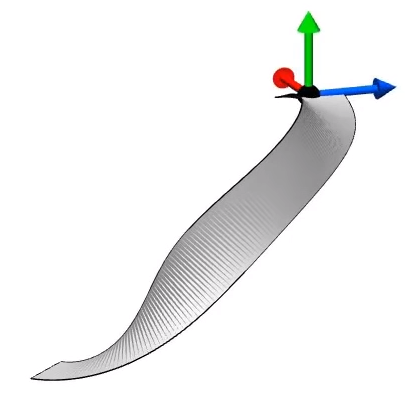
\includegraphics[scale=0.1]{Pictures/noncontractiblepathbelt.png} \\
        $\updownarrow$ & $\updownarrow$ & $\updownarrow$ \\
        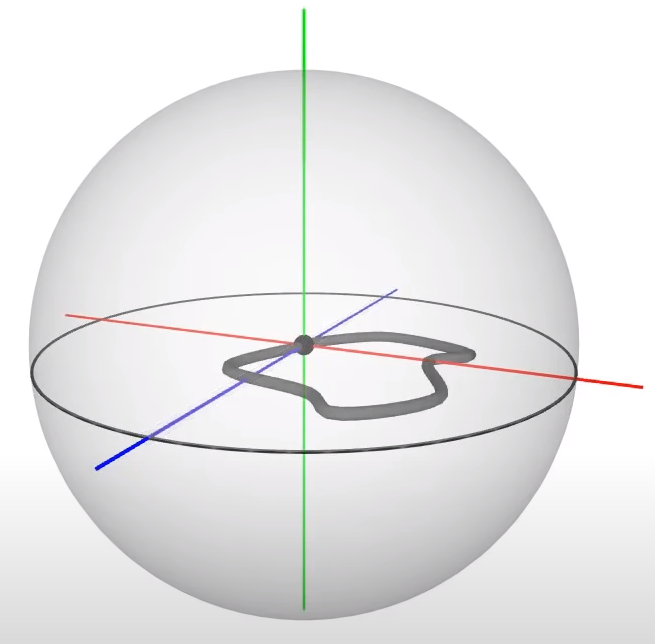
\includegraphics[scale=0.1]{Pictures/randomrotsphere.png} & 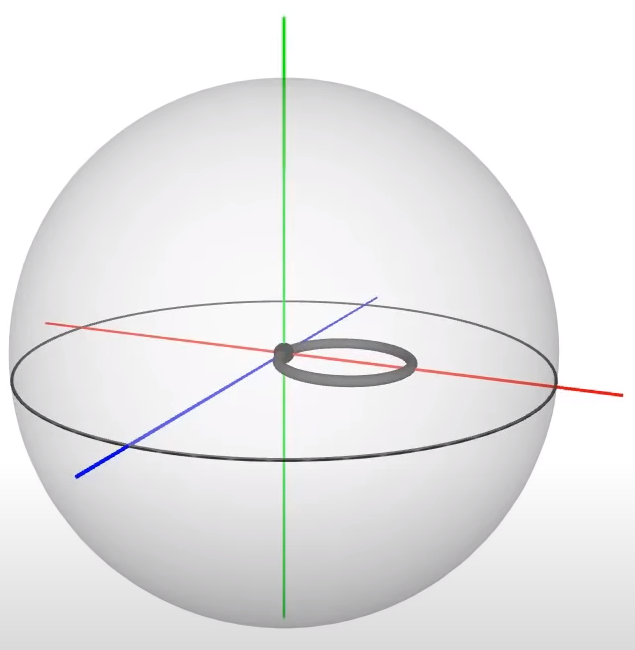
\includegraphics[scale=0.08]{Pictures/contractiblepathsphere.png} & 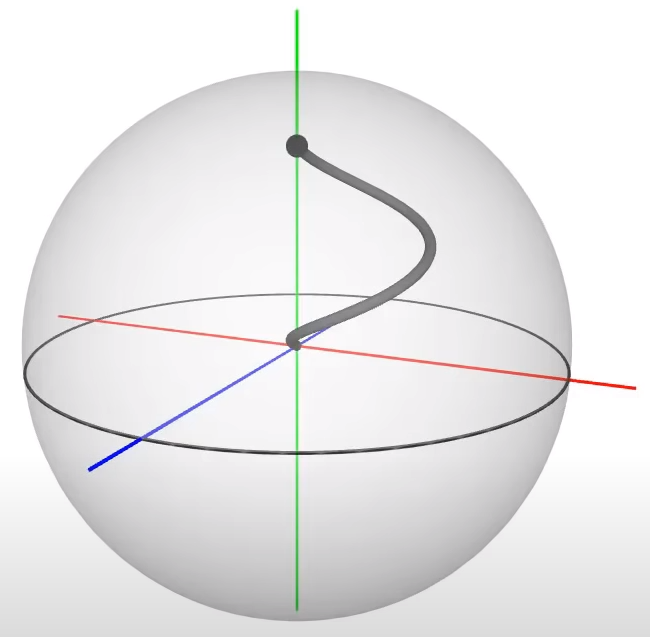
\includegraphics[scale=0.08]{Pictures/noncontractiblepathsphere.png}
    \end{tabular}
  \end{center}
\end{frame}

\begin{frame}{Dictionary}
    \begin{center}
    \begin{tabular}{|ccc|}
        \hline
        \textbf{\underline{Belt}} & & \textbf{\underline{Path}} \\[0.2cm]
        specific configuration & $\longleftrightarrow$ & specific path \\[0.2cm]
        moving the ends & $\longleftrightarrow$ & continuous deformation  \\[0.2cm]
        ends have same orientation & $\longleftrightarrow$ & closed path (loop) \\[0.2cm]
        \emph{can be flattened} & $\longleftrightarrow$ & \emph{contractible} \\ \hline
    \end{tabular}
    \end{center}
    \textbf{Back to Dirac's belt trick:}
    \begin{enumerate}
      \item ends of the belt have same orientation \textcolor{blue}{$\to$ we consider loops} \\
      \hspace{5.8cm} {\tiny \textcolor{blue}{(passing through the origin)}}
      \item moving the ends of the belt \textcolor{blue}{$\to$ continuous deformation} \\
      \item belt in original (flat) position \textcolor{blue}{$\to$ trivial path}
    \end{enumerate}
    The question then becomes: \textbf{which loops are contractible ?}
\end{frame}

\begin{frame}{Problem solved ?}
    \begin{itemize}
      \item \textbf{\underline{$4\pi$-twist:}}
    We saw in the beginning the the $4\pi$-twist can be flattened, how can we see this in terms of paths ?
    \begin{center}
        \begin{tabular}{m{2cm} m{0.5cm} m{2cm} m{0.5cm} m{2cm}}
            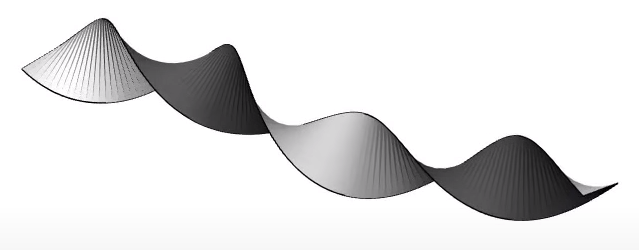
\includegraphics[scale=0.1]{Pictures/4pibelt.png} & $\longleftrightarrow$ & 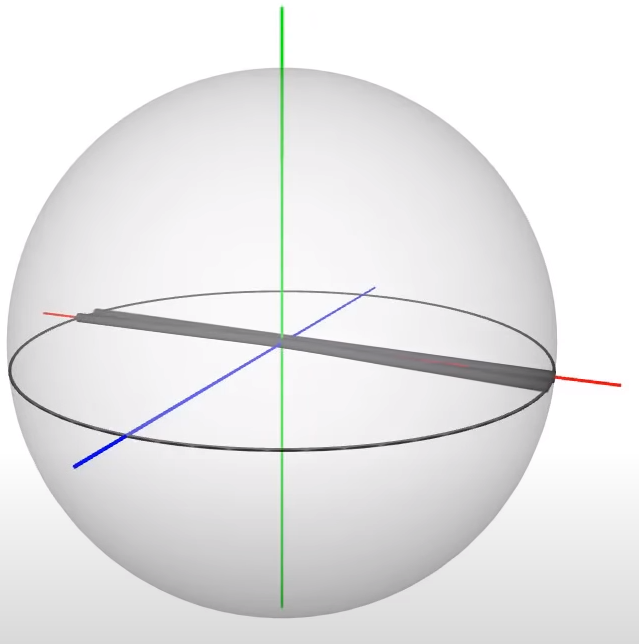
\includegraphics[scale=0.08]{Pictures/4pisphere1.png} & $\longrightarrow$ & 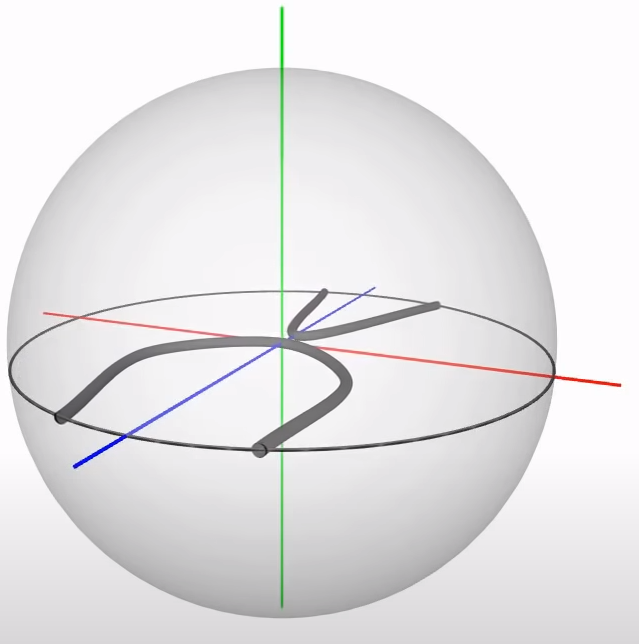
\includegraphics[scale=0.08]{Pictures/4pisphere2.png} \\
            & & & & \hspace{0.7cm} $\downarrow$ \\
            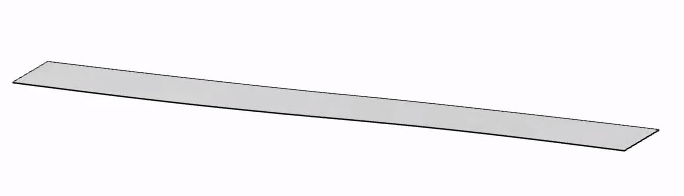
\includegraphics[scale=0.1]{Pictures/flatbelt.png} & $\longleftrightarrow$ & 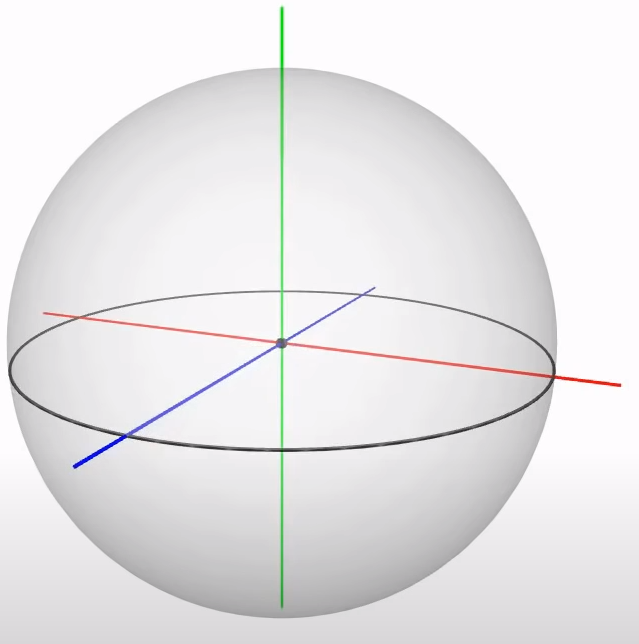
\includegraphics[scale=0.08]{Pictures/4pisphere4.png} & $\longleftarrow$ & 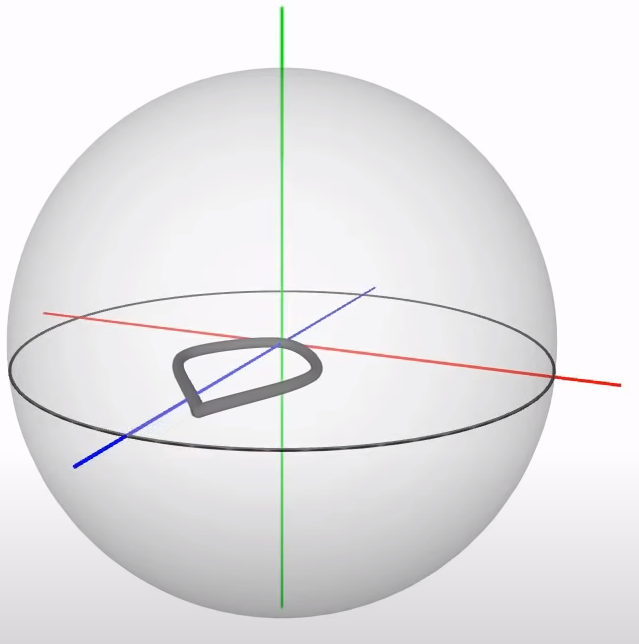
\includegraphics[scale=0.08]{Pictures/4pisphere3.png}
        \end{tabular}
    \end{center}
    $\Rightarrow$ the $4\pi$-twist is \emph{contractible} ! Great.
    \item \textbf{\underline{$2\pi$-twist:}} we ``clearly'' see that is not contractible... no ?! Great..?..  \\[0.2cm]
  \end{itemize}
  \textbf{Wierd aftertaste:} our ``proof'' is good to show contractibility but bad to show non-contractibility and it only works for simple examples.\\
  $\Rightarrow$ We want a consistent and general way of studying paths in topological spaces.
\end{frame}

\section{Homotopy theory}

\begin{frame}{Homotopoy theory primer}
    \textbf{Starting observation:} depending on the topological space, all loops might not be contractible. Moreover, some loops are ``fundamentally different'' from each other.\\
    Examples: $\R^3$, $S^2$, $\mathbb{T}^2$, etc.

    \begin{block}{Paths and homotopies}
         For a topological space $X$:
        \begin{itemize}
          \item \textit{Path} in $X$: continuous map $\gamma:[0,1]\to X$, \textit{loop} if closed
          \item $\gamma_1$ and $\gamma_2$ are \textit{homotopically equivalent} if one can be deformed into the other: there exists
          $H:[0,1]\times [0,1]\to X$ such that
          \begin{equation*}
              H(0,t)=\gamma_1(t)\qquad \text{and}\qquad H(1,t)=\gamma_2(t).
          \end{equation*}
          This is an equivalence relation ($\sim$).
        \end{itemize}
    \end{block}
    
    For each $x_0\in X$, we define
    \begin{equation*}
        \pi_1(X,x_0) = \{\text{all loops based at }x_0\}/\sim,
    \end{equation*}
    it is the set of ``fundamentally different'' loops passing through $x_0$.
\end{frame}

\begin{frame}{Fundamental group}
    Group structure on $\pi_1(X,x_0)$:
    \begin{itemize}
      \item \textbf{Product} of paths: $\gamma_1\cdot\gamma_2=$ ``$\gamma_1$ then $\gamma_2$''
      \item \textbf{Inverse} path: $\gamma^{-1}=$ ``$\gamma$ traversed in the opposite direction''
      \item \textbf{Neutral} path: $e=$ ``constant path at the identity''
      \item For equivalence classes: $[\gamma_1]\cdot[\gamma_2]=[\gamma_1\cdot\gamma_2]$ and $[\gamma]^{-1}=[\gamma^{-1}]$
    \end{itemize}
    Important fact: up to isomorphism, $\pi_1(X,x_0)$ does not depend on $x_0$ \\ $\Rightarrow$ we denote it as $\pi_1(X)$, it is called the \emph{fundamental group} of $X$.\\[0.2cm]
    
    Contractible loops are $\sim$ to a point, i.e. they are the element of $[e]$.\\[0.2cm]

    How to compute $\pi_1(X)$ ? Can be difficult, not discussed here.\\[0.2cm]

    \begin{columns}[T,onlytextwidth]
      \column{0.35\textwidth}
        
        \textbf{Examples:}
        \begin{itemize}
          \item $\pi_1(\R^3)=\{e\}$
          \item $\pi_1(S^2) = \{e\}$
          \item $\pi_1(\mathbb{T}^2)=\textcolor{green}{\Z}\times\textcolor{red}{\Z}$
          \item $\pi_1(\R^2\backslash\{p\})=\Z$
        \end{itemize}
  
      \column{0.65\textwidth}
  
        \begin{figure}
          \centering
          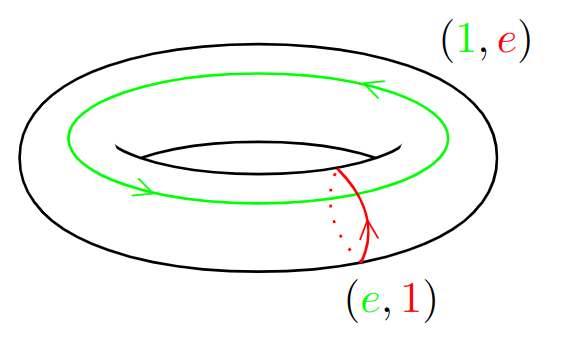
\includegraphics[scale=0.2]{Pictures/torushomotopy3.png}
        \end{figure}
  
    \end{columns}
    Remark: $\pi_1(\R^3\backslash\{p\})=\{e\}$, higher homotopy groups for higher-dimensional holes ?

\end{frame}

\begin{frame}{Back to $\SO(3)$}
    \textbf{Question we had:} are all loops in $\SO(3)$ contractible ?\\
    In homotopy language: is $\pi_1(\SO(3))$ trivial ?\\[0.2cm]
    \textbf{Answer:} \emph{NO}, one can compute that
    \begin{equation*}
        \boxed{\pi_1(\SO(3))=\Z_2}
    \end{equation*}
    $\Rightarrow$ There only two ``fundamentally different'' loops in $\SO(3)$ !\\
    $\Rightarrow$ all non-contractible loops are deformations of the $2\pi$-twist !

    \begin{center}
      \begin{tabular}{|l|}
          \hline
          The belt trick is a way of physically demonstrating that the \\ fundamental group of $\SO(3)$ is $\Z_2$.\\ \hline
      \end{tabular}
    \end{center}

    We can now say, with more confidence, that we understood Dirac's belt trick.\\[0.3cm]

    Are there other manifestation of homotopy in our practical world ?\\[0.3cm]

    Yes: the \emph{spin} ! (Pro: you don't need a belt, Con: you need an electron)\\
    Initially, this trick was a demonstration invented by P. Dirac (1902-1984) to explain the notion of spin to his students.

\end{frame}

\section{Quantum spin and $\SU(2)$}

\section{Conclusion}

\begin{frame}{Blocks}
    Three different block environments are pre-defined and may be styled with an
    optional background color.
  
    \begin{columns}[T,onlytextwidth]
        \column{0.5\textwidth}
          
            Some text.\\[2cm]
            aaaaa
    
        \column{0.5\textwidth}
    
          \begin{block}{Default}
            Block content.
          \end{block}
    
          \begin{alertblock}{Alert}
            Block content.
          \end{alertblock}
    
          \begin{exampleblock}{Example}
            Block content.
          \end{exampleblock}
    
      \end{columns}

  \end{frame}

\appendix

\begin{frame}[fragile]{Backup slides}
  Sometimes, it is useful to add slides at the end of your presentation to
  refer to during audience questions.

  The best way to do this is to include the \verb|appendixnumberbeamer|
  package in your preamble and call \verb|\appendix| before your backup slides.

  \themename will automatically turn off slide numbering and progress bars for
  slides in the appendix.  \cite{ConcreteMath}
\end{frame}

\begin{frame}[allowframebreaks]{References}

  \bibliography{bibliography}
  \bibliographystyle{abbrv}

\end{frame}

\end{document}
